% Figure snippets for BELA manuscript. Include after Stage 3 writing.

\begin{figure}[htbp]
\centering

\includegraphics[width=0.95\textwidth]{figures/fig_pipeline.pdf}
\caption{Overview of the BELA pipeline. Day-5 time-lapse frames (96--112 hpi)
are processed into 512-dimensional feature vectors by a pre-trained VGG16
backbone. A multitask bidirectional LSTM jointly predicts inner cell mass
(ICM), trophectoderm (TE), expansion score, and the overall blastocyst score.
The resulting model-derived blastocyst score (MDBS) is combined with maternal
age in a logistic regression to predict ploidy status.}
\label{fig:pipeline}
\end{figure}

\begin{figure}[htbp]
\centering
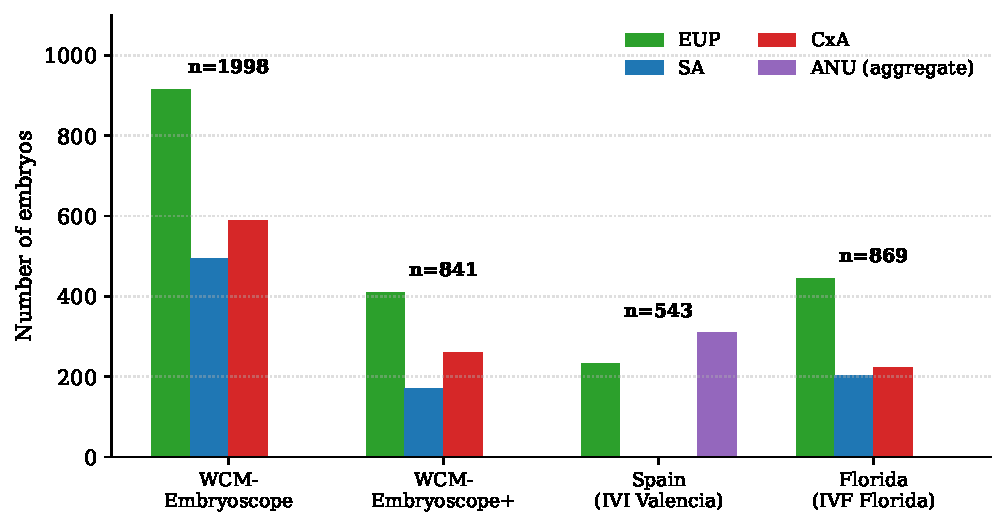
\includegraphics[width=0.72\textwidth]{figures/fig_datasets.pdf}
\caption{Characteristics of the four datasets used in this study. WCM-Embryoscope
(1{,}998 embryos), WCM-Embryoscope+ (841 embryos), Spain/IVI Valencia
(543 embryos), and Florida/IVF Florida (869 embryos). The Spain dataset reports
aneuploidy as a single aggregate class (ANU), while WCM and Florida report
single aneuploid (SA) and complex aneuploid (CxA) subcategories in addition
to euploid (EUP).}
\label{fig:datasets}
\end{figure}

\begin{figure}[htbp]
\centering
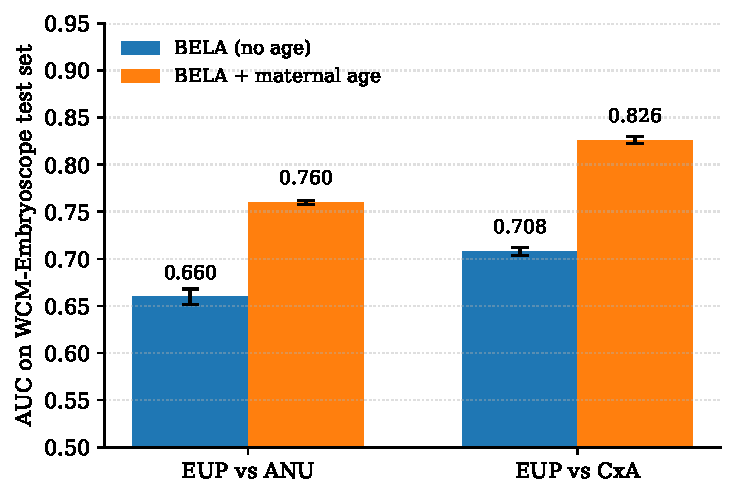
\includegraphics[width=0.72\textwidth]{figures/fig_auc_wcm.pdf}
\caption{BELA ploidy classification AUC on the WCM-Embryoscope test set with
and without inclusion of maternal age. For the EUP~vs~ANU task, AUC rises from
0.66~$\pm$~0.008 to 0.76~$\pm$~0.002 when maternal age is included. For the
EUP~vs~CxA task, AUC rises from 0.708~$\pm$~0.004 to 0.826~$\pm$~0.004.
Error bars denote standard errors across cross-validation folds.}
\label{fig:auc_wcm}
\end{figure}

\begin{figure}[htbp]
\centering
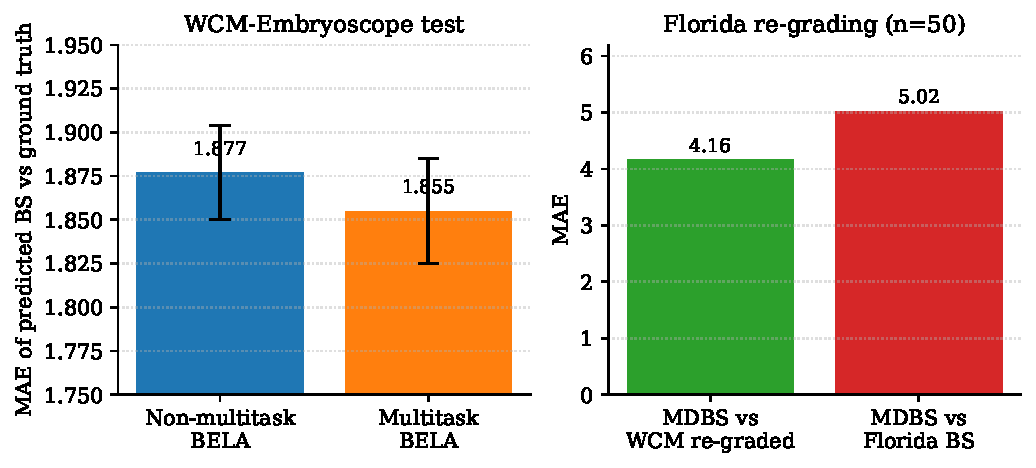
\includegraphics[width=0.95\textwidth]{figures/fig_mae_comparisons.pdf}
\caption{(Left) Mean absolute error (MAE) of predicted blastocyst score on
the WCM-Embryoscope test set for multitask BELA (1.855~$\pm$~0.03) and
non-multitask BELA (1.877~$\pm$~0.027). (Right) MAE between the model-derived
blastocyst score (MDBS) and two reference scores on 50 Florida embryos where
the MDBS deviated most strongly from the provided Florida blastocyst scores:
MDBS vs the Weill Cornell re-graded BS (4.16) and MDBS vs the original Florida
BS (5.02).}
\label{fig:mae_comparisons}
\end{figure}

\begin{figure}[htbp]
\centering
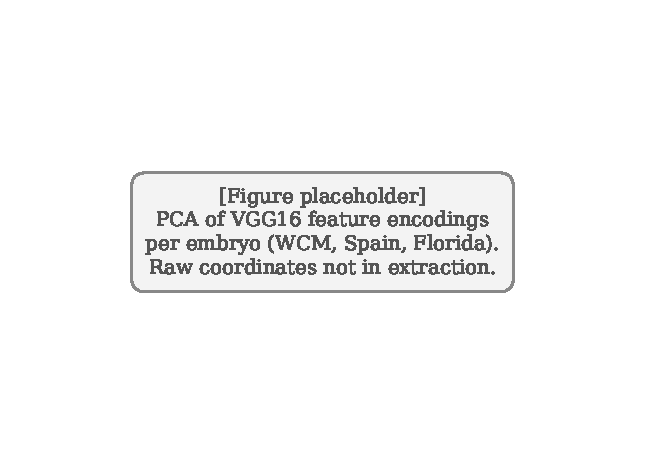
\includegraphics[width=0.5\textwidth]{figures/fig_pca_placeholder.pdf}
\caption{Schematic placeholder for PCA of VGG16 feature encodings of day-5
embryo frames (96--112 hpi) across the WCM-Embryoscope, WCM-Embryoscope+,
Spain, and Florida datasets. Per-embryo coordinates were not available in
the extracted materials used for this manuscript.}
\label{fig:pca_placeholder}
\end{figure}
